\section{Proyecto}
Este programa se desarrolló en APEX de Oracle.
\subsection{Modelo Entidad-Relación}
El modelo Entidad-Relación (ER) de la figura \ref{fig:modelo-er} nos permite presentar la estructura del proyecto de modo que sea entendido por la mayoría de personas.
\begin{figure}[H]
  \centering
  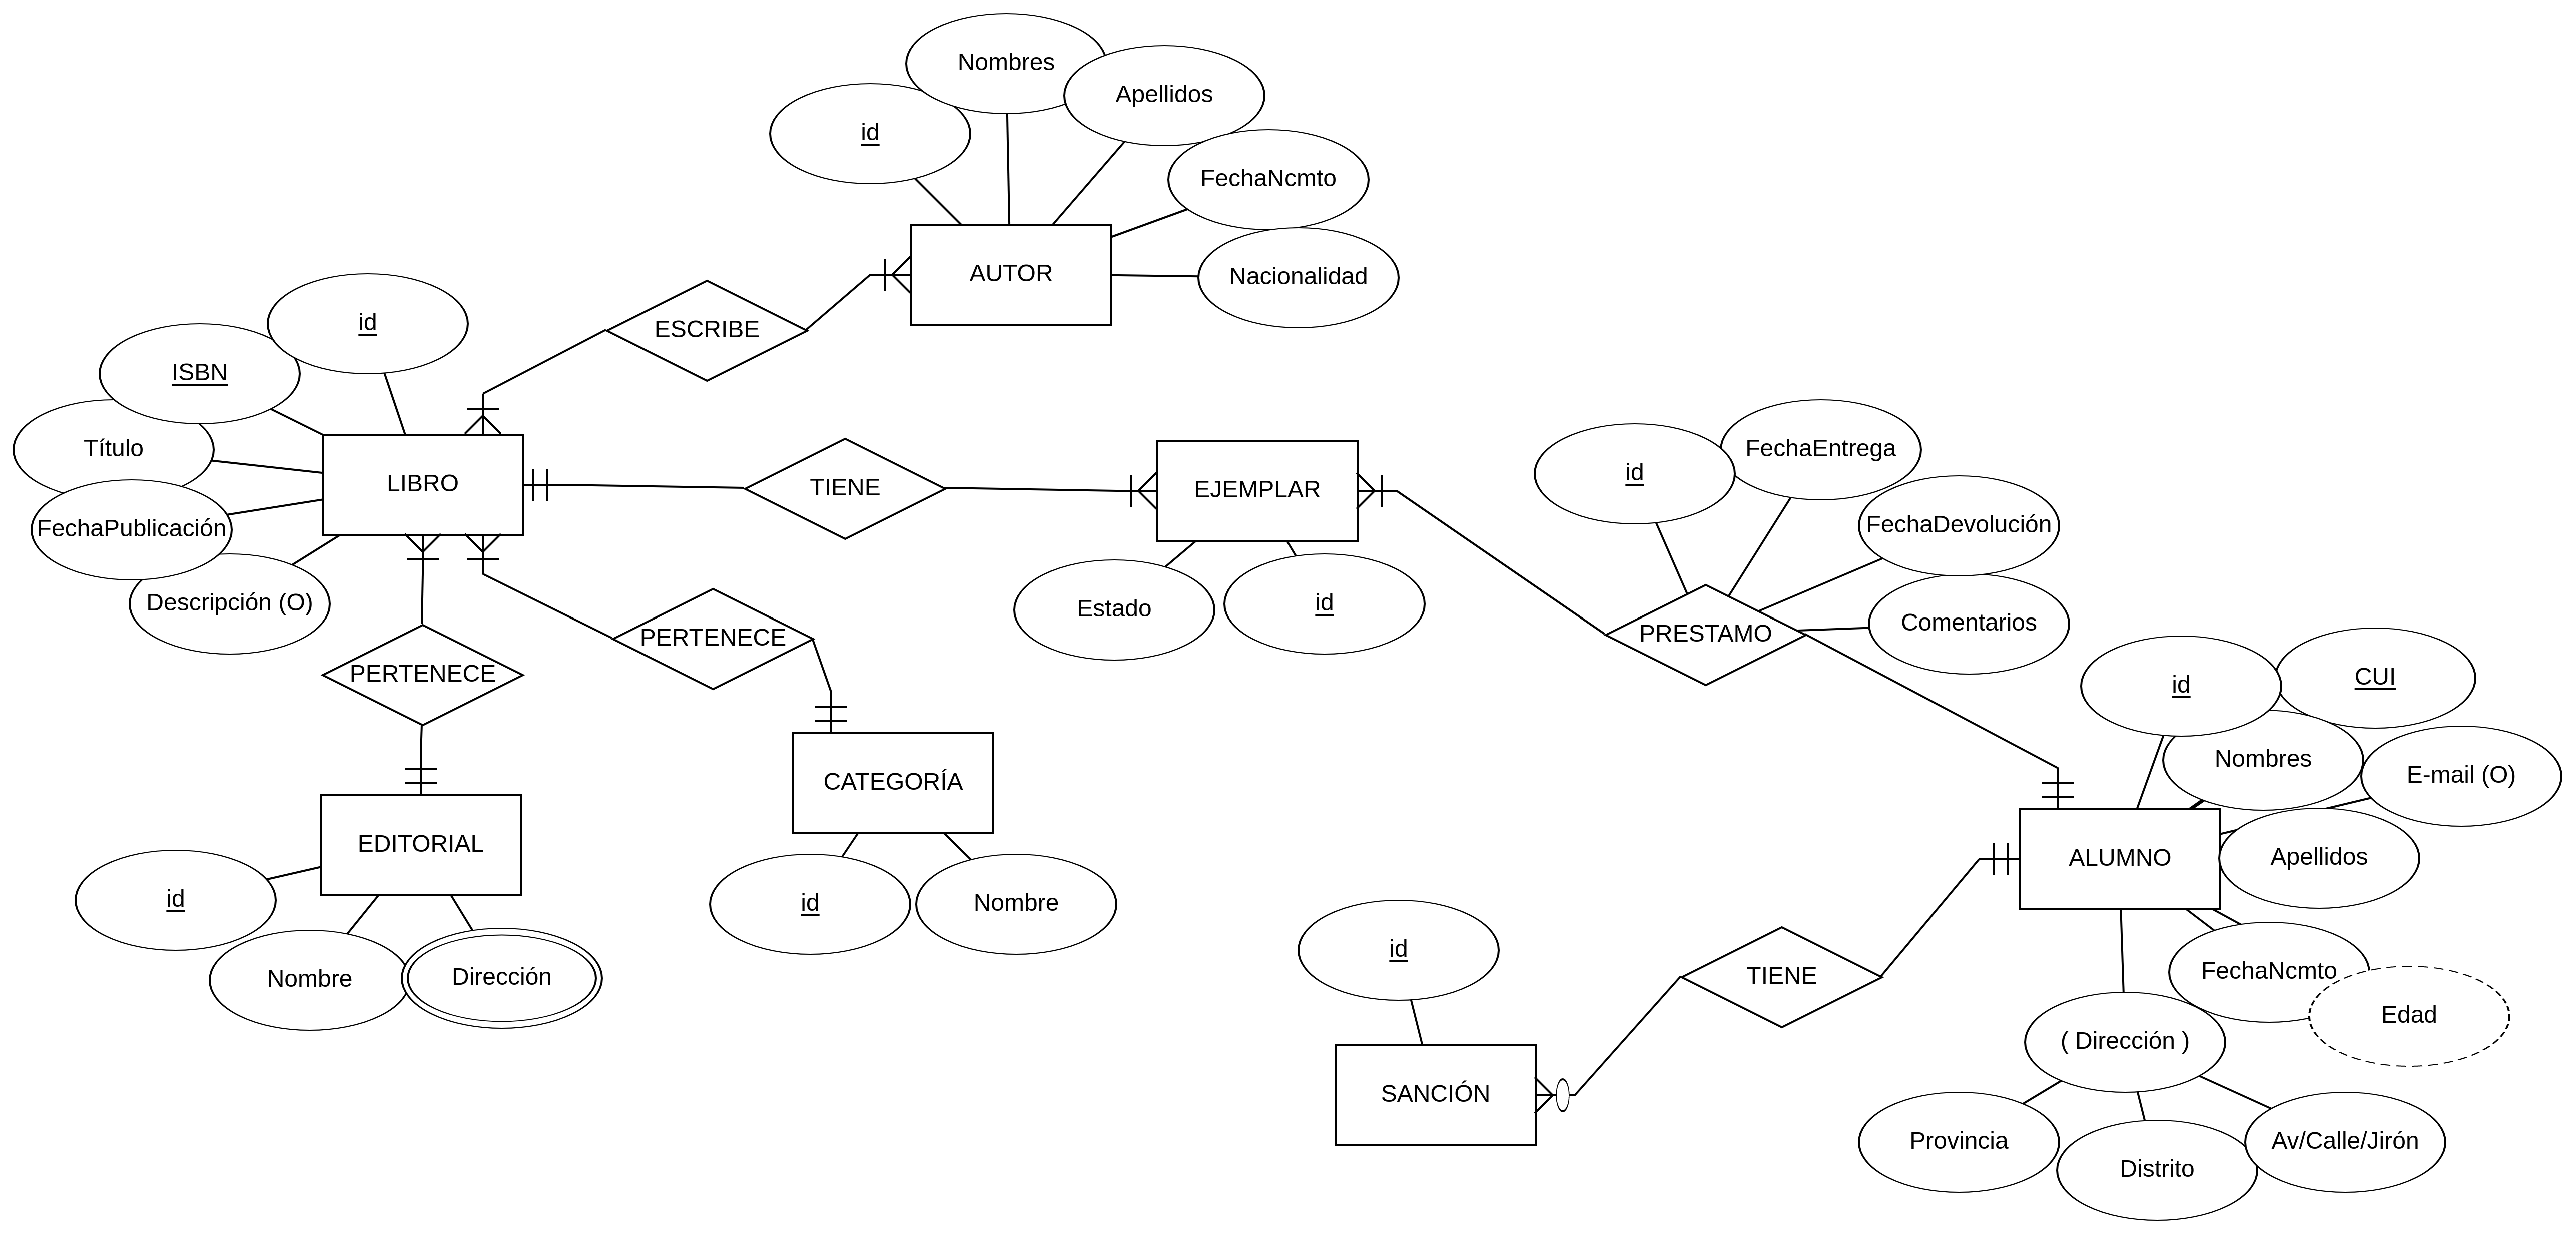
\includegraphics[width=0.95\textwidth]{modelo-er}
  \caption{Modelo Entidad-Relación}
  \label{fig:modelo-er}
\end{figure}

\subsection{Modelo Relacional}
El modelo Relacional de la figura \ref{fig:modelo-relacional} es una vista lógica, porque muestra como las entidades se relacionan entre sí.
\begin{figure}[H]
  \centering
  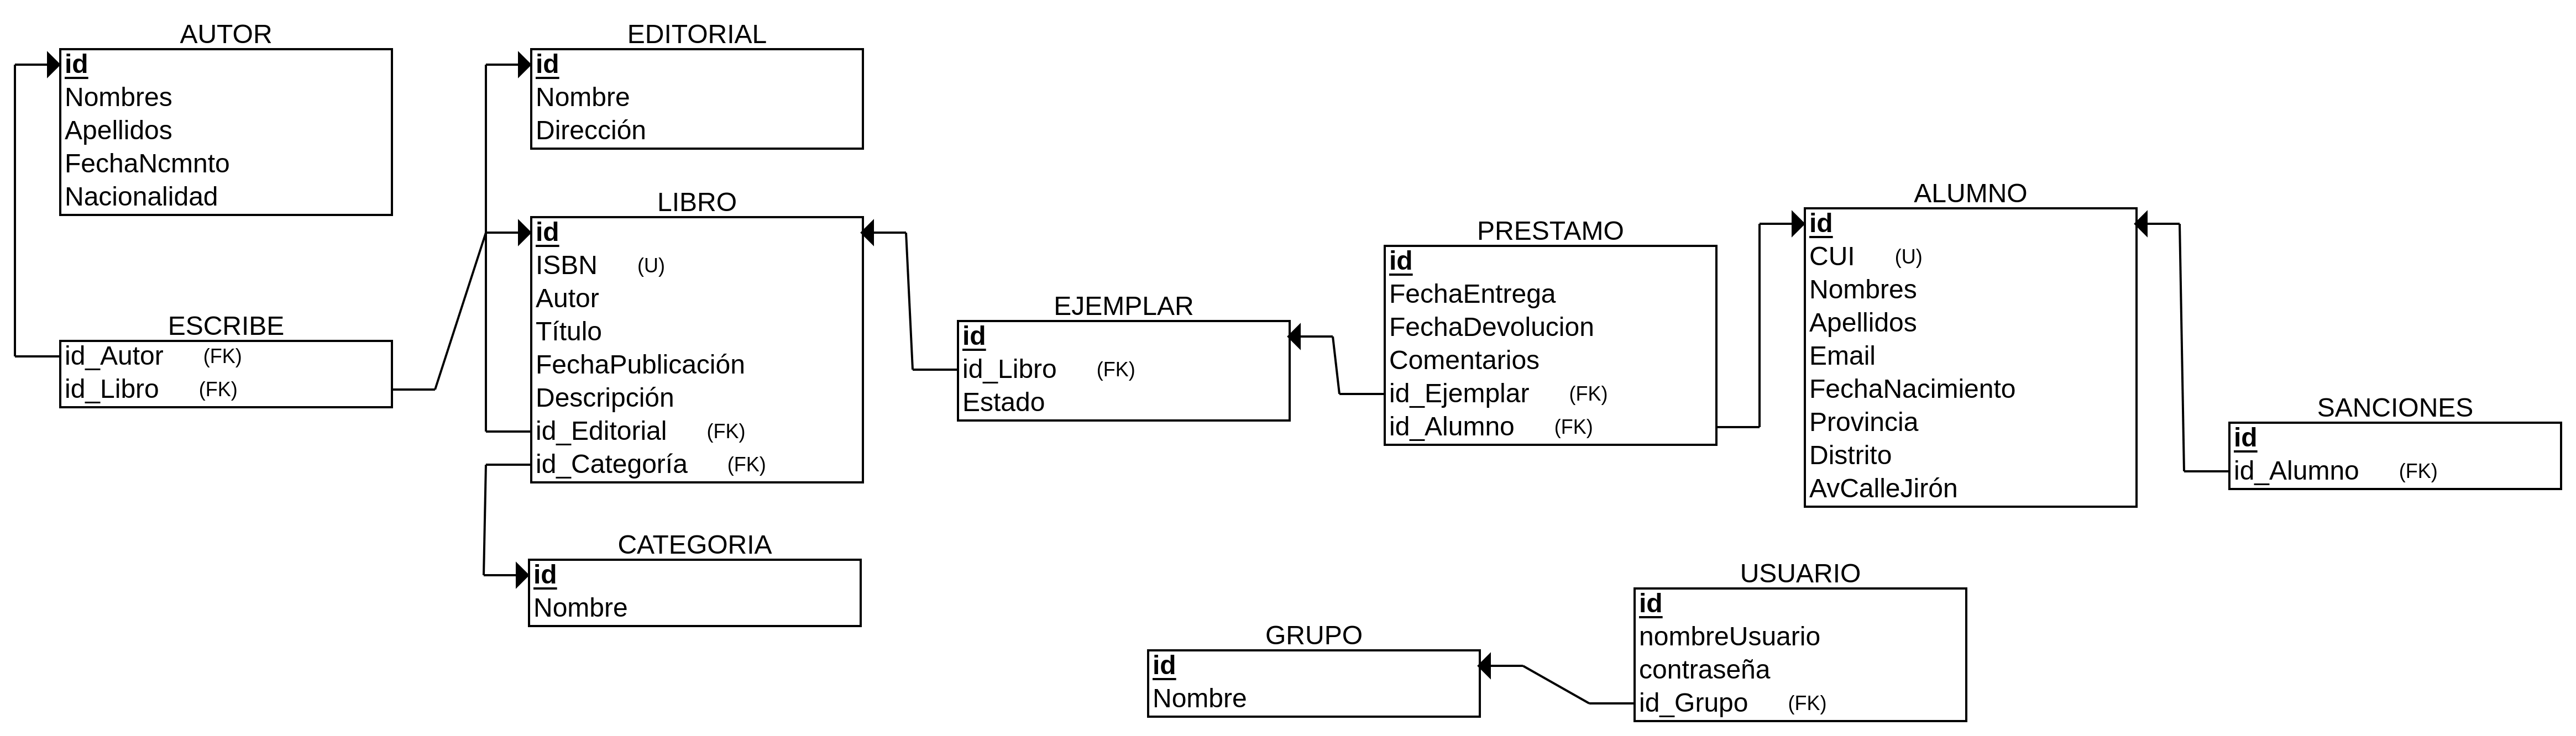
\includegraphics[width=0.95\textwidth]{modelo-relacional}
  \caption{Modelo Relacional}
  \label{fig:modelo-relacional}
\end{figure}

\subsection{Código SQL}
\lstinputlisting[language=SQL]{../../../src/sql/biblioteca.sql}

Para la segunda revisión del proyecto se agregaron las tablas \textit{Autor} y \textit{Escribe} porque un libro puede tener varios autores. Así mismo se creo una función que cambia el \textit{estado} de un libro cuando este es prestado.
\lstinputlisting[language=SQL]{../../../src/sql/rev2.sql}